% !TEX program = LuaTeX
\documentclass{article}
\usepackage{forest}
\usepackage{float}
\usepackage{colortbl}
\usetikzlibrary{shadows,arrows.meta}
\usepackage[a4paper, total={190mm, 277mm}]{geometry}
\usepackage{fontspec}
%\setmainfont{TimesNewRoman}

\begin{document}
  \begin{figure}[H]
    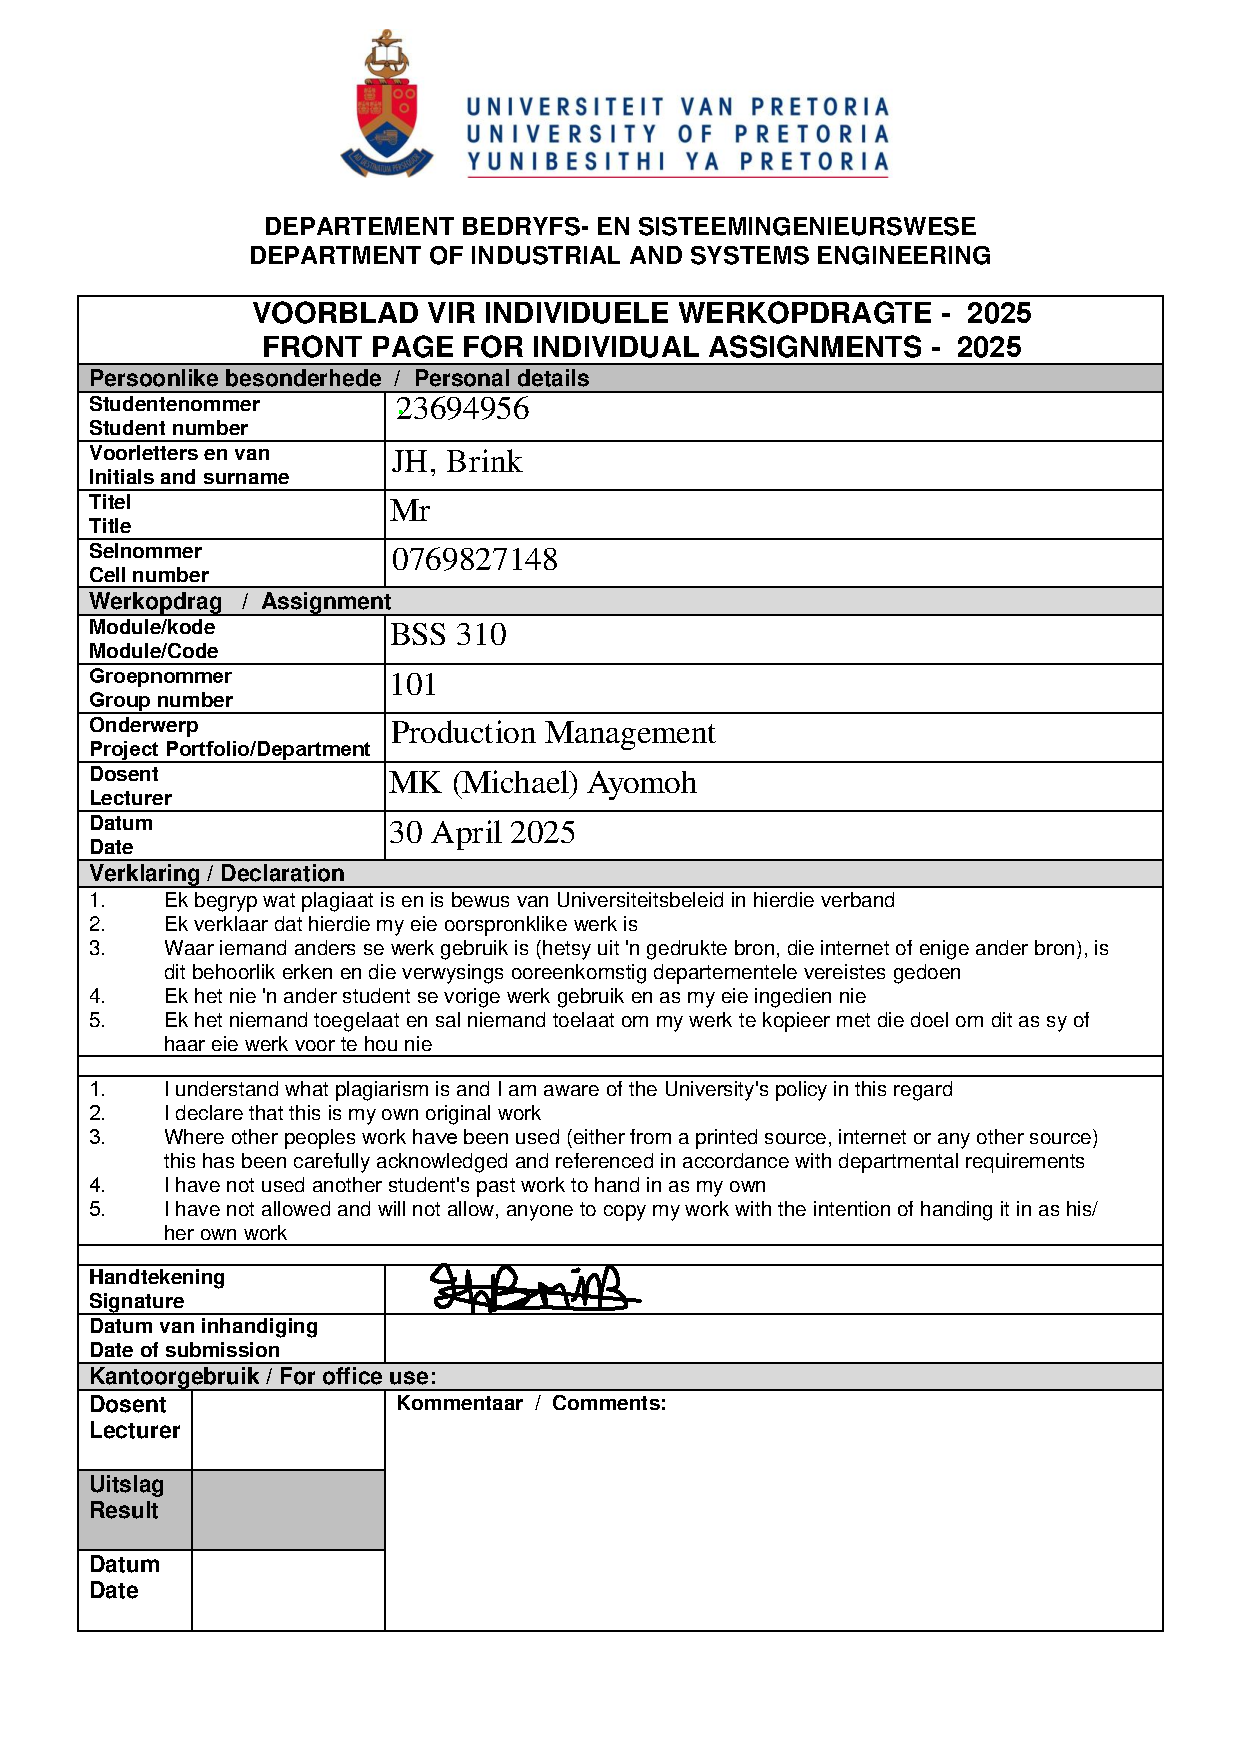
\includegraphics[width=1\linewidth]{figures/Cover_Page_Part_B_Jan-Hendrik.pdf}
  \end{figure}
  \newpage{}
  \huge{
    \bfseries{
    PART B - Production Management\\
    (Jan-Hendrik Brink u23694956)
    }
  }
\Large
  \section{Description of system characteristics based on functional
  capabilities} 
  The Production system is designed to be cost-effective and capable to
  produce portable, durable and
  professionally aesthetic ADHD stimulating chair attachments through a
  combination of diligent material sourcing, a optimized automated
  manufacturing process, having parts conform to global standards, and
  thoughtful design of components such as interlocking joints and final 
  finish. 
  \section{Project scope and stakeholders}
  \subsection{Project scope}
  The project's overarching goal is to create an affordable, Portable, Durable
  and professionally aesthetic chair attachment for the comfort and stimulation
  of ADHD sufferers. The product needs to address the limitations of existing
solutions by being noise free, allowing the use of both hands and being easily
  transportable. The project needs to deliver on providing adequate stimulation
  for ADHD sufferers and significantly increasing the time spent on On-task
  activities. As well as being cost-effective, targeting availability to middle-class
  customers. Key requirements being careful material sourcing, optimized
  manufacturing system, parts that conform to strict standardization. Notable
  exclusions from the production system scope is the large
  scale retail distrobution and material production. Materials will be sourced
  via third party dealers and distributors will be handled by the Logistics
  system.
  \subsection{Project stakeholders}
  \begin{table}[H]
    \Large
    \centering
    \caption{Table of Internal and External Stakeholders for Production}
  \begin{tabular}{|l|l|}
    \hline
    \textbf{Internal Stakeholders} & \textbf{External Stakeholders}  \\
    \hline
      Jan-Hendrik (Production Manager)    & Material Supplier \\
      Supervisory Employees               & Paint Supplier \\
      IT and System Managers              & Silicone Coating Supplier \\
      Factory Employees                   & Valves Supplier \\
                                          & Machinery Supplier \\
                                          & Machinery Servicer \\
                                          & Drill Supplier \\
      \hline
  \end{tabular}
  \end{table}
  %\begin{center}
  %  \textit{Figure 1.1 : Table of Internal and External Stakeholders}
  %\end{center}
  \begin{figure}[H]
  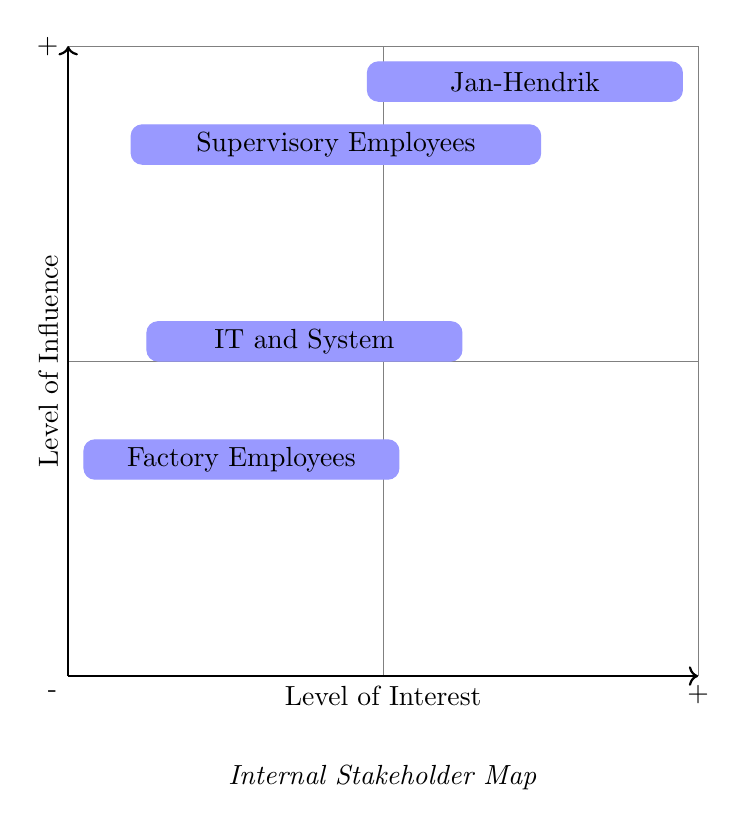
\begin{tikzpicture}
    \draw[step=4cm,gray,very thin] (0,0) grid (8,8);
    \draw[thick,->] (0,0) -- (8,0) node[anchor=south,left=4cm,below] {Level of
    Interest} node[anchor=south,left=4cm,below=1cm] {\textit{Internal Stakeholder Map}};
    \draw[thick,->] (0,0) -- (0,8) node[anchor=south,above=-4cm,rotate=90] {Level of Influence};
    \draw (0,0) node[left=0.2cm,below] {-};
    \draw (8,0) node[anchor=north,below] {+};
    \draw (0,8) node[anchor=east] {+};
    
    \newcommand{\JIT}{7.8}
    \newcommand{\JIF}{7.8}
    \draw[rounded corners,fill=blue!40,draw=blue!40] (\JIT-4, \JIF-0.5) rectangle
    (\JIT,\JIF) (\JIT-2,\JIF-0.25) node[anchor=center] {Jan-Hendrik};
    
    \newcommand{\SEIT}{6}
    \newcommand{\SEIF}{7}
    \draw[rounded corners,fill=blue!40,draw=blue!40] (\SEIT-5.2, \SEIF-0.5) rectangle
    (\SEIT,\SEIF) (\SEIT-2.6,\SEIF-0.25) node[anchor=center] {Supervisory Employees};
    
    \newcommand{\ITIT}{5}
    \newcommand{\ITIF}{4.5}
    \draw[rounded corners,fill=blue!40,draw=blue!40] (\ITIT-4,\ITIF-0.5) rectangle
    (\ITIT,\ITIF) (\ITIT-2,\ITIF-0.25) node[anchor=center] {IT and System};
    
    \newcommand{\FEIT}{4.2}
    \newcommand{\FEIF}{3}
    \draw[rounded corners,fill=blue!40,draw=blue!40] (\FEIT-4, \FEIF-0.5) rectangle
    (\FEIT,\FEIF) (\FEIT-2,\FEIF-0.25) node[anchor=center] {Factory Employees};
  \end{tikzpicture}
  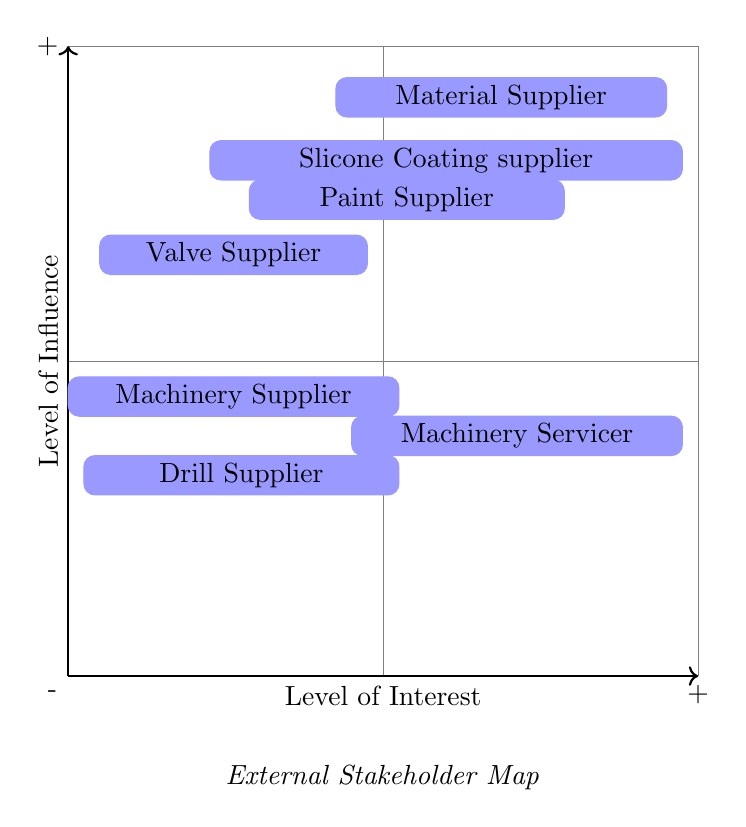
\begin{tikzpicture}
    \draw[step=4cm,gray,very thin] (0,0) grid (8,8);
    \draw[thick,->] (0,0) -- (8,0) node[anchor=south,left=4cm,below] {Level of
    Interest} node[anchor=south,left=4cm,below=1cm] {\textit{External Stakeholder Map}};
    \draw[thick,->] (0,0) -- (0,8) node[anchor=south,above=-4cm,rotate=90] {Level of Influence};
    \draw (0,0) node[left=0.2cm,below] {-};
    \draw (8,0) node[anchor=north,below] {+};
    \draw (0,8) node[anchor=east] {+};
 
    \newcommand{\MatIT}{7.6}
    \newcommand{\MatIF}{7.6}
    \draw[rounded corners,fill=blue!40,draw=blue!40] (\MatIT-4.2, \MatIF-0.5) rectangle
    (\MatIT,\MatIF) (\MatIT-2.1,\MatIF-0.25) node[anchor=center] {Material Supplier};

    \newcommand{\PSIT}{6.3}
    \newcommand{\PSIF}{6.3}
    \draw[rounded corners,fill=blue!40,draw=blue!40] (\PSIT-4, \PSIF-0.5) rectangle
    (\PSIT,\PSIF) (\PSIT-2,\PSIF-0.25) node[anchor=center] {Paint Supplier};

    \newcommand{\SSIT}{6.8}
    \newcommand{\SSIF}{6.8}
    \draw[rounded corners,fill=blue!40,draw=blue!40] (\SSIT-5, \SSIF-0.5) rectangle
    (\SSIT+1,\SSIF) (\SSIT-2,\SSIF-0.25) node[anchor=center] {Slicone Coating
    supplier};

    \newcommand{\VSIT}{4.1}
    \newcommand{\VSIF}{5.6}
    \draw[rounded corners,fill=blue!40,draw=blue!40] (\VSIT-3.7, \VSIF-0.5) rectangle
    (\VSIT-0.3,\VSIF) (\VSIT-2,\VSIF-0.25) node[anchor=center] {Valve Supplier};

    \newcommand{\MacIT}{4.2}
    \newcommand{\MacIF}{3.8}
    \draw[rounded corners,fill=blue!40,draw=blue!40] (\MacIT-4.2, \MacIF-0.5) rectangle
    (\MacIT,\MacIF) (\MacIT-2.1,\MacIF-0.25) node[anchor=center] {Machinery Supplier};

    \newcommand{\MasIT}{7.8}
    \newcommand{\MasIF}{3.3}
    \draw[rounded corners,fill=blue!40,draw=blue!40] (\MasIT-4.2, \MasIF-0.5) rectangle
    (\MasIT,\MasIF) (\MasIT-2.1,\MasIF-0.25) node[anchor=center] {Machinery Servicer};

    \newcommand{\DSIT}{4.2}
    \newcommand{\DSIF}{2.8}
    \draw[rounded corners,fill=blue!40,draw=blue!40] (\DSIT-4, \DSIF-0.5) rectangle
    (\DSIT,\DSIF) (\DSIT-2,\DSIF-0.25) node[anchor=center] {Drill Supplier};

  \end{tikzpicture}
    \caption{Internal and External stakeholder map for production}

  \end{figure}
  \section{Project Plan}
  \subsection{Phases and deliverables}

  \begin{enumerate}
    \item \textbf{Planning Phase:} \\
      Project Plan is formally defined based on the stated problem and
      objectives. The Plan is then reviewed and adapted if necessary. \\
      \textbf{Deliverables:}
      \begin{itemize}
        \item Project scope and objective documents.
        \item Risk assessment documents.
        \item Stakeholder register and communication plan is submitted.
        \item Initial requirements documents.
        \item Financial capital. 
        \item Identified target market.
        \item Feasibility reports. 
        \item ADHD stimulation research report. 
        \item Material suitability research report. 
        \item Detailed product design.
        \item Technical drawings of product parts.
        \item Packaging designs.
        \item Prototype materials. 
        \item Functional prototype. 
        \item Prototype performance testing reports. 
      \end{itemize}
    \item \textbf{Production Phase:} \\
      Mass production starts \\
      \textbf{Deliverables:}
      \begin{itemize}
        \item Supplier contracts. 
        \item Functional manufacturing process. 
        \item Acquired production machinery. 
        \item Fully set-up factory. 
        \item Detailed Quality control process. 
        \item batch of products. 
        \item Quality conformance report of batch of products. 
      \end{itemize}
    \item \textbf{Reflection Phase:} \\
      \textbf{Deliverables:}
      \begin{itemize}
        \item Distributor feedback reports. 
        \item Customer feedback reports. 
        \item Detailed Product weaknesses list. 
        \item detailed product improvement plan. 
        \item Improved product design. 
        \item Improved manufacturing process. 
      \end{itemize}
  \end{enumerate}


  \subsection{Work Breakdown Structure (WBS)}
    \small
    \begin{figure}[H]
      \centering
      \tikzset{
        every node/.style={draw,text width=0cm},
        style1/.style= {text width=10cm,rectangle, rounded corners=2pt, thin,align=center,fill=green!30},
        style2/.style= {text width=3cm,rectangle, rounded corners=6pt, thin,align=center,fill=green!60},
        style3/.style= {text width=2cm,outer sep=0cm,rectangle, rounded corners=6pt, thin,align=left,fill=green!90},
        style4/.style= {text width=2cm,rectangle,thin,align=left,fill=pink!60}
      }
      \begin{tikzpicture}[
        remember picture,
        level 1/.style={sibling distance=5.2cm},
        level 2/.style={sibling distance=2.6cm},
        edge from parent/.style={->,draw},
        >=latex]
        % the initial tree ("root" and "text nodes")
        \node[style1] {ADHD chair attachment Project} 
          child {node[style2] (a) {Planning Phase}
            child {node[style3] (a1) {A1. Initialization}}
            child {node[style3] (a2) {A2. Research}}
            child {node[style3] (a3) {A3. Prototype}}
          }
          child {node[style2,xshift=1.3cm] (b) {Production Phase}
            child {node[style3] (b1) {B1. Production System }}
            child {node[style3] (b2) {B2. Quality Control }}
          }
          child {node[style2,xshift=1.3cm] (c) {Reflection Phase}
            child {node[style3] (c1) {C1. Feedback Collection}}
            child {node[style3] (c2) {C2. Feedback Implementation}}
          };
        
       % the nodes below each of the "subline" nodes
        %A 
        \node [style4,below of = a1,xshift=6pt,yshift=-15pt] (a11) 
        {A1.1 Define project scope and objective};
        \node [style4,below of = a11,yshift=-25pt] (a12)
        {A1.2 Conduct initial risk assesement};
        \node [style4,below of = a12,yshift=-32pt] (a13)
        {A1.3 Establish stakeholders and communication plan};
        \node [style4,below of = a13,yshift=-27pt] (a14)
        {A1.4 Analyze initial requirements};
        \node [style4,below of = a14,yshift=-27pt] (a15)
        {A1.5 Aquire financial capital (bank or investors)};
        \node [style4,below of = a15,yshift=-39pt] (a16)
        {A1.6 Monitor project progress according to plan};
      
        \node [style4,below of = a2,xshift=6pt,yshift=-8pt] (a21) 
        {A2.1 Identify target market};
        \node [style4,below of = a21,yshift=-13pt] (a22)
        {A2.2 Analyze existing solutions};
        \node [style4,below of = a22,yshift=-20pt] (a23)
        {A2.3 Conduct feasability study};
        \node [style4,below of = a23,yshift=-33pt] (a24)
        {A2.4 Research ADHD stimulation requirements};
        \node [style4,below of = a24,yshift=-32pt] (a25)
        {A2.5 Research for suitable materials};
        \node [style4,below of = a25,yshift=-26pt] (a26)
        {A2.6 Create detailed product design};
        \node [style4,below of = a26,yshift=-33pt] (a27)
        {A2.7 Draw technical drawings for product parts};
        \node [style4,below of = a27,yshift=-32pt] (a28)
        {A2.8 Design packaging and use guidelines};

        \node [style4,below of = a3,xshift=6pt,yshift=-8pt] (a31) 
        {A3.1 Source prototype materials};
        \node [style4,below of = a31,yshift=-20pt] (a32)
        {A3.2 Fabricate functional prototype};
        \node [style4,below of = a32,yshift=-20pt] (a33)
        {A3.3 Coduct performance testing};
        \node [style4,below of = a33,yshift=-28pt] (a34)
        {A3.4 Conduct material cost analysis per part};
        \node [style4,below of = a34,yshift=-32pt] (a35)
        {A3.5 Assess material quality conformance};
        \node [style4,below of = a35,yshift=-26pt] (a36)
        {A3.6 Measure production time per part};
        \node [style4,below of = a36,yshift=-21pt] (a37)
        {A3.7 Test joint duty cycle};
        \node [style4,below of = a37,yshift=-15pt] (a38)
        {A3.8 Test Paint adhesion strength};
        \node [style4,below of = a38,yshift=-14pt] (a39)
        {A3.9 Analyze testing results};
        \node [style4,below of = a39,yshift=-20pt] (a310)
        {A3.10 Revise design based on testing feedback};


      
        % B 
      
        \node [style4,below of = b1,xshift=6pt,yshift=-27pt] (b11) 
        {B1.1 Identify material, machinery and paint suppliers};
        \node [style4,below of = b11,yshift=-31pt] (b12)
        {B1.2 Establish supplier contracts};
        \node [style4,below of = b12,yshift=-15pt] (b13)
        {B1.3 Design manufacturing process};
        \node [style4,below of = b13,yshift=-21pt] (b14)
        {B1.4 Acquire and Install production machinery};
        \node [style4,below of = b14,yshift=-26pt] (b15)
        {B1.5 Implement automation software};
        \node [style4,below of = b15,yshift=-20pt] (b16)
        {B1.6 Establish inventory system};
        \node [style4,below of = b16,yshift=-15pt] (b17)
        {B1.7 Set up factory layout};
      
        \node [style4,below of = b2,xshift=6pt,yshift=-14pt] (b21) 
        {B2.1 Setup Quality control procedures};
        \node [style4,below of = b21,yshift=-20pt] (b22)
        {B2.2 Produce first batch};
        \node [style4,below of = b22,yshift=-20pt] (b23) 
        {B2.3 Monitor and test manufacturing process};
        \node [style4,below of = b23,yshift=-26pt] (b24)
        {B2.4 Perform quality checks on first batch};
        \node [style4,below of = b24,yshift=-21pt] (b25)
        {B2.5 Create quality report};
        \node [style4,below of = b25,yshift=-15pt] (b26) 
        {B2.6 Analyze quality report};
        \node [style4,below of = b26,yshift=-27pt] (b27)
        {B2.7 Refine manufacturing process based on report};
        \node [style4,below of = b27,yshift=-32pt] (b28)
        {B2.8 Ship product batch dealers};
      
        %C 
      
        \node [style4,below of = c1,xshift=6pt,yshift=-20pt] (c11) 
        {C1.1 Collect sales and distrobution information};
        \node [style4,below of = c11,yshift=-25pt] (c12)
        {C1.2 Collect distrobutor and cutomer feedback};
        \node [style4,below of = c12,yshift=-20pt] (c13)
        {C1.3 Monitor product lifecycle};
        \node [style4,below of = c13,yshift=-15pt] (c14)
        {C1.4 Create product usage reports};
        \node [style4,below of = c14,yshift=-16pt] (c15)
        {C1.5 Analyze product usage report};
        \node [style4,below of = c15,yshift=-15pt] (c16)
        {C1.6 Identify product weaknesses};
        \node [style4,below of = c16,yshift=-21pt] (c17)
        {C1.7 Identify possible product improvements};
      
        \node [style4,below of = c2,xshift=6pt,yshift=-26pt] (c21)
        {C2.1 Implement identified product improvements};
        \node [style4,below of = c21,yshift=-33pt] (c22)
        {C2.2 Redesign worst performing parts};
        \node [style4,below of = c22,yshift=-28pt] (c23)
        {C2.3 Re-evaluate manufacturing process};
        \node [style4,below of = c23,yshift=-34pt] (c24)
        {C2.4 Implement changes to add part improvements};
        \node [style4,below of = c24,yshift=-38pt] (c25)
        {C2.5 Redesign product with improved parts in mind};
        \node [style4,below of = c25,yshift=-45pt] (c26)
        {C2.6 Return to Planning Prototype Phase using improved design};
        \node [style4,below of = c26,yshift=-34pt] (c27)
        {C2.7 Manufacture new design};
        \node [style4,below of = c27,yshift=-22pt] (c28)
        {C2.8 Perform Quality control on new design};
        \node [style4,below of = c28,yshift=-22pt] (c29)
        {C2.9 Collect feedback on new design};
        \node [style4,below of = c29,yshift=-21pt] (c210)
        {C2.10 Interate on new design using feedback};






        % lines from each "text" node to every one of its "children"
        \foreach \value in {1,...,6}
        \draw[->] (a1.195) |- (a1\value.west);
      
        \foreach \value in {1,...,8}
        \draw[->] (a2.195) |- (a2\value.west);

        \foreach \value in {1,...,10}
        \draw[->] (a3.195) |- (a3\value.west);
      
        \foreach \value in {1,...,7}
        \draw[->] (b1.195) |- (b1\value.west);
      
        \foreach \value in {1,...,8}
        \draw[->] (b2.195) |- (b2\value.west);
      
        \foreach \value in {1,...,7}
        \draw[->] (c1.195) |- (c1\value.west);
      
        \foreach \value in {1,...,10}
        \draw[->] (c2.195) |- (c2\value.west);
      
      \end{tikzpicture}
      \caption{Work Breakdown Structure for production}
    \end{figure}
    \Large

  \subsection{Network Diagram}
    \tikzset{
      every node/.style={},
      style1/.style= {draw,text width=1cm,rectangle,align=center},
      stylea1/.style= {draw,text width=1cm,rectangle,align=center,fill=green!10},
      stylea2/.style= {draw,text width=1cm,rectangle,align=center,fill=green!20},
      stylea3/.style= {draw,text width=1cm,rectangle,align=center,fill=green!30},
      styleb1/.style= {draw,text width=1cm,rectangle,align=center,fill=blue!10},
      styleb2/.style= {draw,text width=1cm,rectangle,align=center,fill=blue!20},
      stylec1/.style= {draw,text width=1cm,rectangle,align=center,fill=red!10},
      stylec2/.style= {draw,text width=1cm,rectangle,align=center,fill=red!20},
      stylecp/.style= {thick,draw=red!256},
    }
    \begin{figure}[H]
      \scriptsize
      \begin{tikzpicture}[
        node distance=1.5cm,
        ]
        \newcommand{\tab}{\ \ \ \ };

        \node[stylea1] (A11) 
        {0 \tab 1 \\ A1.1 \\ 1 \\ 7 \tab 8};
        \node[stylea1,right of = A11] (A15)
        {1 \tab 10 \\ A1.5 \\ 10 \\ 98 \ \ 108};
        \node[stylea2,right of = A15] (A24) 
        {10 \tab 15 \\ A2.4 \\ 5 \\ 108  113};

        \node[stylea2,right of = A24] (A26) 
        {15 \tab 18 \\ A2.6 \\ 3 \\ 113  116};
        \node[right of = A26] (S1) {};

        \node[styleb2,above of = A26] (B21)
        {15 \tab 20 \\ B2.1 \\ 5 \\ 113  118};

        \node[styleb1,below of = A26] (B11) 
        {15 \tab 18 \\ B1.1 \\ 3 \\ 113 116};
        \node[styleb1,right of = B11] (B12) 
        {18 \tab 21 \\ B1.2 \\ 3 \\ 128 131};

        \node[styleb1,below of = B11] (B13) 
        {15 \tab 20 \\ B1.3 \\ 5 \\ 113 118};
        \node[styleb1,right of = B13] (B16) 
        {20 \tab 23 \\ B1.6 \\ 3 \\ 118 121};
        \node[styleb1,right of = B16] (B17) 
        {23 \tab 37 \\ B1.7 \\ 14 \\ 121 135};

        \node[stylea3,right of = S1] (A31) 
        {21 \tab 25 \\ A3.1 \\ 4 \\ 131 135};
        \node[stylea3,right of = A31] (A32) 
        {25 \tab 27  \\ A3.2 \\ 2 \\ 135 137};

        \node[styleb2,right of = A32] (B23) 
        {37 \tab 40 \\ B2.3 \\ 3 \\ 137 140};
        \node[styleb2,right of = B23] (B24) 
        {40 \tab 42 \\ B2.4 \\ 2 \\ 140 142};
        \node[styleb2,right of = B24] (B28) 
        {42 \tab 43 \\ B2.8 \\ 1 \\ 142 143};

        \node[stylec1,right of = B28] (C12)
        {71 \tab 79 \\ C1.2 \\ 8 \\ 171 179};
        \node[stylec1,above of = C12] (C11) 
        {71 \tab 77 \\ C1.1 \\ 6 \\ 171 177};
        \node[stylec1,below of = C12] (C13)
        {43 \tab 73 \\ C1.3 \\ 30 \\ 143 173};

        \node[stylec1,right of = C12] (C16)
        {79 \tab 83  \\ C1.6 \\ 4 \\ 179 183};
        \node[stylec2,right of = C16] (C21)
        {83 \tab 93  \\ C2.1 \\ 10 \\ 183 193};
       
        \draw[stylecp,->] (A11.east) -- (A15.west); 
        \draw[stylecp,->] (A11.east) -- (A15.west); 
        \draw[stylecp,->] (A15.east) -- (A24.west); 
        \draw[->] (A24.east) -- (A26.west);
        \draw[->] (A26.east) -- (A31.west);
        \draw[->] (A31.east) -- (A32.west);
        \draw[->] (A32.east) -- (B23.west);
        \draw[stylecp,->] (B23.east) -- (B24.west);
        \draw[stylecp,->] (B24.east) -- (B28.west);
        \draw[stylecp,->] (B28.east) -- (C12.west);
        \draw[stylecp,->] (C12.east) -- (C16.west);
        \draw[stylecp,->] (C16.east) -- (C21.west);

        \draw[->] (B11.east) -- (B12.west);

        \draw[stylecp,->] (B13.east) -- (B16.west);
        \draw[stylecp,->] (B16.east) -- (B17.west);

        \draw (3.7cm,0cm) -- (3.7cm,1.5cm);
        \draw[stylecp] (A24.east) -- (3.7cm,0cm);
        \draw[->] (3.7cm,1.5cm) -- (B21.west);
        \draw[->] (3.7cm,-1.5cm) -- (B11.west);

        \draw[stylecp] (3.7cm,0cm) -- (3.7cm,-3cm);
        \draw[stylecp,->] (3.7cm,-3cm) -- (B13.west);

        \draw (6.7cm,-1.5cm) -- (6.7cm,0cm);
        \draw (B12.east) -- (6.7cm,-1.5cm);

        \draw[stylecp] (9.75cm,-3cm) -- (9.75cm,0cm);
        \draw[stylecp] (B17.east) -- (9.75cm,-3cm);
        \draw[stylecp,->] (9.75cm,0cm) -- (B23.west);

        \draw (9.75cm,1.5cm) -- (9.75cm,0cm);
        \draw (B21.east) -- (9.75cm,1.5cm);

        \draw (14.19cm,1.5cm) -- (14.19cm,-1.5cm); 
        \draw[->] (14.19cm,1.5cm) -- (C11.west);
        \draw[->] (14.19cm,-1.5cm) -- (C13.west);

        \draw (15.72cm,1.5cm) -- (15.72cm,-1.5cm); 
        \draw (C11.east) -- (15.72cm,1.5cm); 
        \draw (C13.east) -- (15.72cm,-1.5cm); 
  
        \draw[stylecp,->] (9.75cm,1.8cm) -- (11.75cm,1.8cm)
        node[above,xshift=-1cm] {Critical Path};

      \end{tikzpicture}
      \caption{Network Diagram for Production}
    \end{figure}

  \subsection{Float, Slack, forward and backward pass}

  \begin{table}[H]
  \caption{Production forward and backward pass table for Production}
  \centering
  \begin{tabular}{|l|l|l|}
    \hline
    & \textbf{Start Date} & \textbf{Finish Date}  \\
    \hline
        \textbf{Forward Pass} & 4 May 2025 & 5 August 2025 \\
    \hline
        \textbf{Backward Pass} & 11 May 2025 & 20 November 2025 \\
    \hline
  \end{tabular}
  \end{table}
  \begin{table}[H]
    \caption{Float and Slack Table for Production}
    \centering
    \Large
  \begin{tabular}{|l|l|l|}
    \hline
    \textbf{Activity} & \textbf{Float} & \textbf{Slack}  \\ \hline
        \rowcolor{green!10} A1.1 & 7 & 0 \\ \hline
        \rowcolor{green!10} A1.5 & 98  &  0 \\ \hline
        \rowcolor{green!20} A2.4 & 98  &  0 \\ \hline
        \rowcolor{green!20} A2.6 & 98  &  3 \\ \hline
        \rowcolor{blue!10} B2.1 & 98  & 17 \\ \hline
        \rowcolor{blue!10} B1.1 & 98  &  0 \\ \hline
        \rowcolor{blue!10} B1.2 & 110 &  0 \\ \hline
        \rowcolor{blue!10} B1.3 & 98  &  0 \\ \hline
        \rowcolor{blue!10} B1.6 & 98  &  0 \\ \hline
        \rowcolor{blue!10} B1.7 & 98  &  0 \\ \hline
        %\multicolumn{3}{c}{\textit{Figure 4.2 Production}} \\
        %\multicolumn{3}{c}{\textit{Float and Slack Table Part A}}

  \end{tabular}
  \begin{tabular}{|l|l|l|}
    \hline
    \textbf{Activity} & \textbf{Float} & \textbf{Slack}  \\ \hline  
      \rowcolor{green!30} A3.1 & 110 & 0 \\ \hline
      \rowcolor{green!30} A3.2 & 110 & 0 \\ \hline
      \rowcolor{blue!20}B2.3 & 100 & 0 \\ \hline
      \rowcolor{blue!20}B2.4 & 100 & 0 \\ \hline
      \rowcolor{blue!20}B2.8 & 100 & 0 \\ \hline
      \rowcolor{red!10}C1.1 & 100 & 2 \\ \hline
      \rowcolor{red!10}C1.2 & 100 & 0 \\ \hline
      \rowcolor{red!10}C1.3 & 100 & 6 \\ \hline
      \rowcolor{red!10}C1.6 & 100 & 0 \\ \hline
      \rowcolor{red!20}C2.1 & 100 & 0 \\ \hline
      %\multicolumn{3}{c}{\textit{Figure 4.3 Production}} \\
      %\multicolumn{3}{c}{\textit{Float and Slack Table Part B}}

  \end{tabular} 
  \end{table}

  \subsection{Key Performance Indicators (KPI's)}

  \begin{table}[H]
    \caption{Key Performance Indicator's table for Production}
    \Large
    \begin{tabular}{ |p{3cm}|p{10.5cm}|p{4cm}| } \hline
      \textbf{KPI} & \textbf{Description} & \textbf{Goal} \\ \hline

      \multicolumn{3}{|c|}{\textbf{Performance Indicators for Material Sourcing}} \\ \hline

      Material Cost Variance &
      Measure deviation from target cost to actual cost of materials &
      Target cost as close as possible to actual cost.
      \begin{math} \frac{actual \ cost}{target \ cost} \le 1 \end{math} \\
      \hline
      On-Time material delivery rate &
      Percentage of material deliveries that arrive on time or earlier than expected
      date. &
      \ge 90\% \\
      \hline
      Material quality conformance rate &
      percentage of sources materials that meet quality requirements &
      \ge 95\% \\
      \hline

      \multicolumn{3}{|c|}{\textbf{Performance Indicators for Manufacturing
      Process}} \\ \hline

      Manufacturing time per unit &
      Measure average time to produce a single unit. &
      As small as possible without compromising production reliability \\
      \hline
      Machine downtime &
      Time machines spend due to maintenance or failures relative to scheduled
      up time. &
      \le 5\% \\
      \hline
      Automated steps &
      Percentage of processes or steps automated in the manufacturing process. &
      \begin{math} \frac{automated \ steps}{total \ steps} \times 100 \end{math}
        As high as possible without compromising manufacturing reliability. \\
      \hline

      \multicolumn{3}{|c|}{\textbf{Performance Indicators for Quality control
      process}} \\ \hline

      First time pass rate &
      percentage products manufactured that pass quality checks first time &
      \ge 90\% \\
      \hline
      Defect rate &
      Percentage of products that fail quality checks & 
      \le 5\% \\
      \hline
      Product conformance metrics &
      Paint adhesion score based on the standardized paint adhesion test. Joint
      duty-cycle based on number of full extensions joint can make before
      mechanical failure. Air bag deflation time.
      Dimensional accuracy how accurate the product is to dimensional
      specification. &
      All metrics above minimum set specification \\
      \hline
    \end{tabular}
  \end{table}
  
  \section{Set-Up Budget}

  \begin{table}[H]
    \Large
    \caption{Materials and equipment Budget table for Production}
    \begin{tabular}{|l|l|l|} \hline

      \textbf{Equipment Item} & \textbf{Amount} & \textbf{Cost} \\ \hline
      Drilling machine &     1 & R  62683.13  \\ \hline
      Milling machine &      1 & R  83545.75  \\ \hline
      Special Drill Bit &    1 & R    465.82     \\ \hline
      TIG-welder &           1 & R 124187.58 \\ \hline
      MillerWelds software & 1 & R Included with TIG-welder \\ \hline
      Sewing Machine &       1 & R  22356.00   \\ \hline
      Fabric Cutter &        1 & R 232647.00  \\ \hline
      Spray gun &            2 & R  24219.00  \\ \hline
      Air Compressor &       1 & R  67794.57  \\ \hline 
      \multicolumn{2}{|l|}{\textbf{Equipment Total Cost}} & R 617898.85 \\ 

      \hline
      \hline

      \textbf{Material item} & \textbf{Amount} & \textbf{Cost} \\ \hline
      Aluminium pipe & 800 kg                       & R 43780.5 \\ \hline
      Nylon fabric & 100 $m^2$                      & R 23287.5 \\ \hline
      Air Inflation valve & 400 units               & R  7452.0 \\ \hline 
      Spray Paint & 100 \times 400ml can            & R 11178.0 \\ \hline
      Spray silicone coating & 200 \times 400ml can & R 37260.0 \\ \hline
      Packaging material & 400 $m^2$                & R  6567.0 \\ \hline
      \multicolumn{2}{|l|}{\textbf{Material Total Cost per 400 units}} & R 129525.0 \\ \hline 
    \end{tabular}
  \end{table}

  \begin{table}[H] \Large
    \caption{Human resources Budget table for Production}
    \begin{tabular}{|l|l|l|l|} \hline
      \textbf{Employee} & \textbf{Salary} & \textbf{Number} & \textbf{Cost} \\
      \hline
      Supervisor          & R 15000 p/m & 2 & R 30000 p/m \\ \hline 
      Production worker   & R 7200  p/m & 8 & R 57600 p/m \\ \hline
      Quality inspector   & R 13000 p/m & 3 & R 39000 p/m \\ \hline 
      IT personnel        & R 11500 p/m & 2 & R 23000 p/m \\ \hline 
      Operational Manager & R 30000 p/m & 1 & R 30000 p/m \\ \hline 
      Maintenace worker   & R 21000 p/m & 2 & R 42000 p/m \\ \hline
      Admin Personnel     & R 10500 p/m & 4 & R 42000 p/m \\ \hline 
      \multicolumn{3}{|l|}{\textbf{Human Resources Total Cost}} & R 263600 p/m \\ \hline 
    \end{tabular}
  \end{table}

  \begin{table}[H] \Large
    \caption{Initial Set-Up Budget table for production}
    \begin{tabular}{|l|l|} \hline
      \textbf{Initial Setup Item} & \textbf{Cost} \\ \hline
      \multicolumn{2}{|c|}{\textbf{Once of payment}} \\ \hline
      Equipment           & R 617898.85 \\ \hline
      Warehouse renovation& R 28860     \\ \hline 
      Conveyor belts (8m) & R 18630     \\ \hline 
      trolley jacks (4)    & R 3726      \\ \hline 
      Operational Computer& R 2235.6    \\ \hline
      \multicolumn{2}{|c|}{\textbf{One month}} \\ \hline
      Human resources     & R 263600    \\ \hline
      Materials           & R 129525.0  \\ \hline 
      Warehouse rent      & R 21300     \\ \hline
      Business Insurance  & R 4657.5    \\ \hline 
      Accounting          & R 7000      \\ \hline
      Water costs         & R 4657.5    \\ \hline
      Electrical costs    & R 38812.5   \\ \hline
      \textbf{Set-Up Total Cost} & R 1140902.95 \\ \hline 
    \end{tabular}
  \end{table}

  \section{Project Budget}
  \begin{table}[H] \Large
    \caption{Project Operational Budget Table for Production}
    \begin{tabular}{|l|l|l|l|} \hline
                              & Year 1 & Year 2 & Year 3 \\ \hline 
        Cost of goods         & R 1554300.0 & R 1740816.0 & R 2020590.0 \\ \hline
        Revenue               & R 4800000   & R 5376000.0 & R 6240000.0 \\ \hline
        \textbf{Gross Profit} & R 3245700.0 & R 3635184.0 & R 4219410.0 \\
        \hline
        \hline
        \multicolumn{4}{|c|}{\textbf{Overheads}} \\ \hline
        Warehouse Rent                & R 255600    & R 255600    & R 293940.0  \\ \hline 
        Salaries                      & R 3163200   & R 3163200   & R 3321360.0 \\ \hline
        Accounting fees               & R 84000     & R 84000     & R 88200.0   \\ \hline 
        Insurance fees                & R 55890.0   & R 55890.0   & R 58684.5   \\ \hline
        Unforseen circumstances       & R 50000     & R 50000     & R 50000     \\ \hline
        \textbf{Total Overhead costs} & R 3608690.0 & R 3608690.0 & R 3812184.5 \\
        \hline 
        \hline 
        \textbf{Next Income}          & R-362990.0  & R 26494.0 & R 407225.5 \\ \hline
    \end{tabular}
  \end{table}

\end{document}
